\documentclass{standalone}
\usepackage{tikz}
\usepackage{tikz-cd}
\usepackage{tikz-3dplot}
\usepackage{pgfplots}
\usepackage{pgffor} % For \foreach loop
\pgfplotsset{compat=newest} % Adjust to your version of pgfplots
\def\Circlearrowleft{\ensuremath{%
		\rotatebox[origin=c]{180}{$\circlearrowleft$}}}
\def\Circlearrowright{\ensuremath{%
		\rotatebox[origin=c]{180}{$\circlearrowright$}}}
\def\CircleArrowleft{\ensuremath{%
		\reflectbox{\rotatebox[origin=c]{180}{$\circlearrowleft$}}}}
\def\CircleArrowright{\ensuremath{%
		\reflectbox{\rotatebox[origin=c]{180}{$\circlearrowright$}}}}
\usetikzlibrary{
	3d, % For 3D drawing
	angles,
	arrows,
	arrows.meta,
	backgrounds,
	bending,
	calc,
	decorations.pathmorphing,
	decorations.pathreplacing,
	decorations.markings,
	fit,
	matrix,
	patterns,
	patterns.meta,
	positioning,
	quotes,
	shadows,
	shapes,
	shapes.geometric
}

\begin{document}
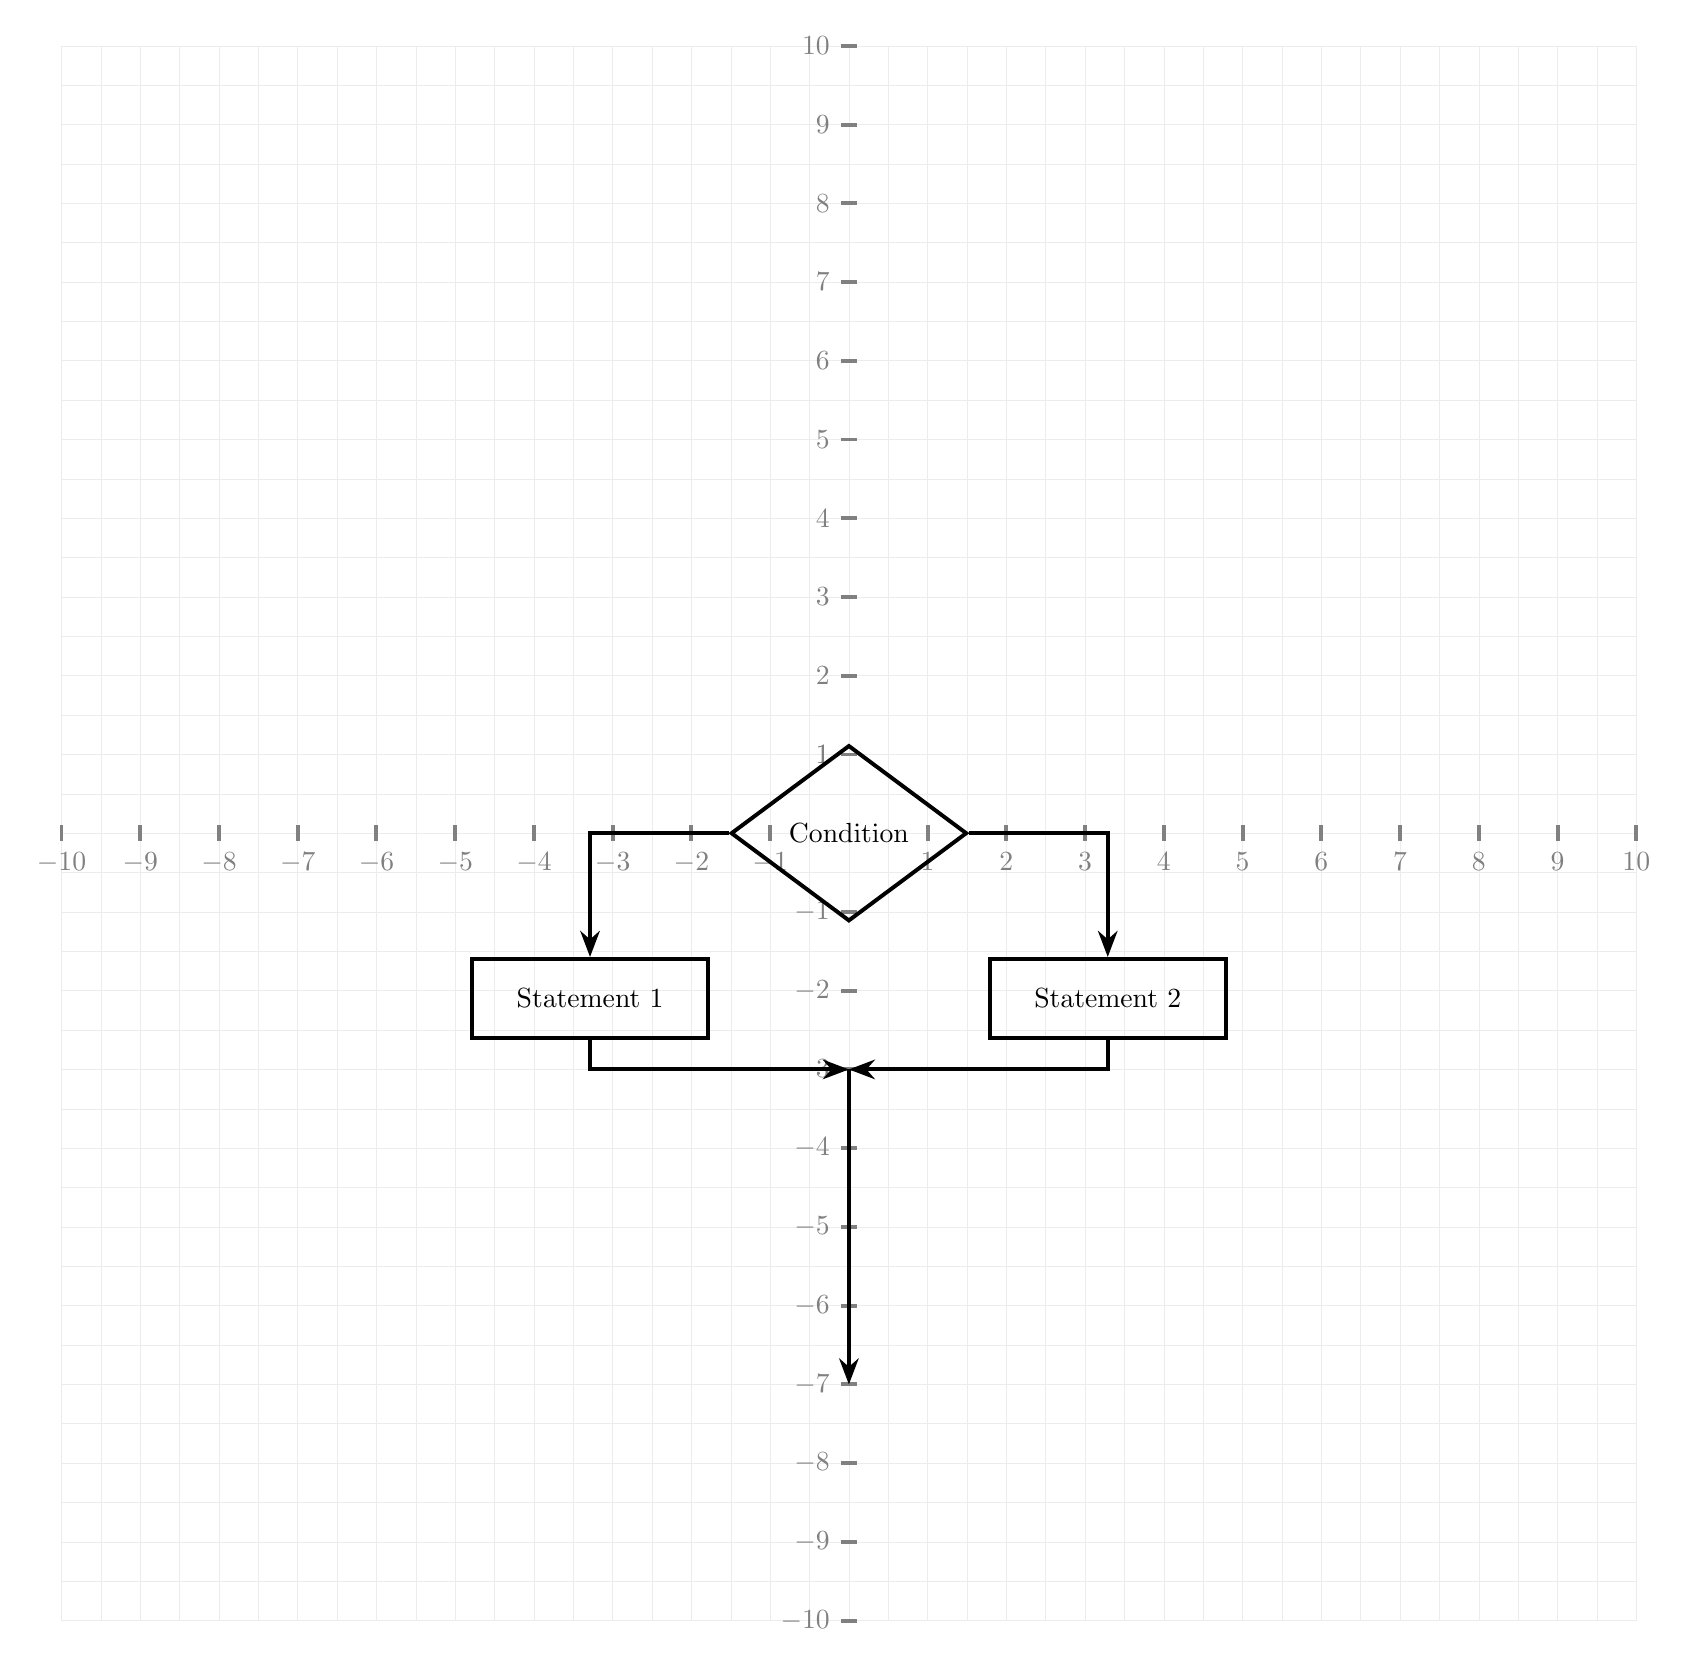
\begin{tikzpicture}[>=Stealth, line width=.5mm]
%	\tikzset{
%	startstop/.style = {rectangle, rounded corners, 
%		minimum width=3cm, 
%		minimum height=1cm,
%		text centered, 
%		draw=black, 
%		fill=red!30},
%	io/.style = {trapezium, 
%		trapezium stretches=true, % A later addition
%		trapezium left angle=70, 
%		trapezium right angle=110, 
%		minimum width=3cm, 
%		minimum height=1cm, text centered, 
%		draw=black, fill=blue!30},
%	process/.style = {rectangle, 
%		minimum width=3cm, 
%		minimum height=1cm, 
%		text centered, 
%		text width=3cm, 
%		draw=black, 
%		fill=orange!30},
%	decision/.style = {diamond, 
%		minimum width=3cm, 
%		minimum height=1cm, 
%		text centered, 
%		draw=black, 
%		fill=green!30}
%	process/.style={rectangle, 
%		minimum width=3cm, 
%		minimum height=1cm, 
%		text centered, 
%		text width=3cm, 
%		draw=black, 
%		fill=orange!30}
%	}

	\def \x{10}
	\def \y{10}
	\draw[very thin,color=gray!15,step=.5] (-\x,-\y) grid (\x,\y);
	
	\foreach \i in {-\x,...,-2,-1,1,2,...,\x}
	\draw[gray] (\i,.1)--(\i,-.1) node[below] {$\i$};%x-axis
	\foreach \i in {-\y,...,-2,-1,1,1,2,...,\y}
	\draw[gray] (.1,\i)--(-.1,\i) node[left] {$\i$};%y-axis
	
%	\node (start) [startstop] {Start};
%	\node (in1) [io, below of=start] {Input};
%	\node (pro1) [process, below of=in1] {Process 1};
	\node (cond) [diamond, 
			minimum width=3cm, 
			minimum height=1cm, 
			text centered,
			draw=black] {Condition};
	\node (state1) [rectangle, 
			minimum width=3cm, 
			minimum height=1cm, 
			text centered, 
			draw=black, 
			below left=of cond] {Statement 1};
	\node (state2) [rectangle, 
			minimum width=3cm, 
			minimum height=1cm, 
			text centered, 
			draw=black, 
			below right=of cond] {Statement 2};
	
	\node (node) [below=2cm of cond] {};

	\draw [->] (cond) -| (state1);
	\draw [->] (cond) -| (state2);
	\draw [->] (state2) |- (0,-3);
	\draw [->] (state1) |- (0,-3);
	\draw [->] (0,-3) -- (0,-7);
%	\draw [->] (in1) -- (pro1);
%	\draw [->] (pro1) -- (dec1);
%	\draw [->] (dec1) -- node[anchor=east] {yes} (pro2a);
%	\draw [->] (dec1) -- node[anchor=south] {no} (pro2b);
%	\draw [->] (pro2b) |- (pro1);
%	\draw [->] (pro2a) -- (out1);
%	\draw [->] (out1) -- (stop);
	
\end{tikzpicture}
\end{document}
